\subsection{VOILA Achieves Pareto-Optimal Trade-offs}
\label{sec:pareto_analysis}

\begin{figure*}[t]
    \centering
    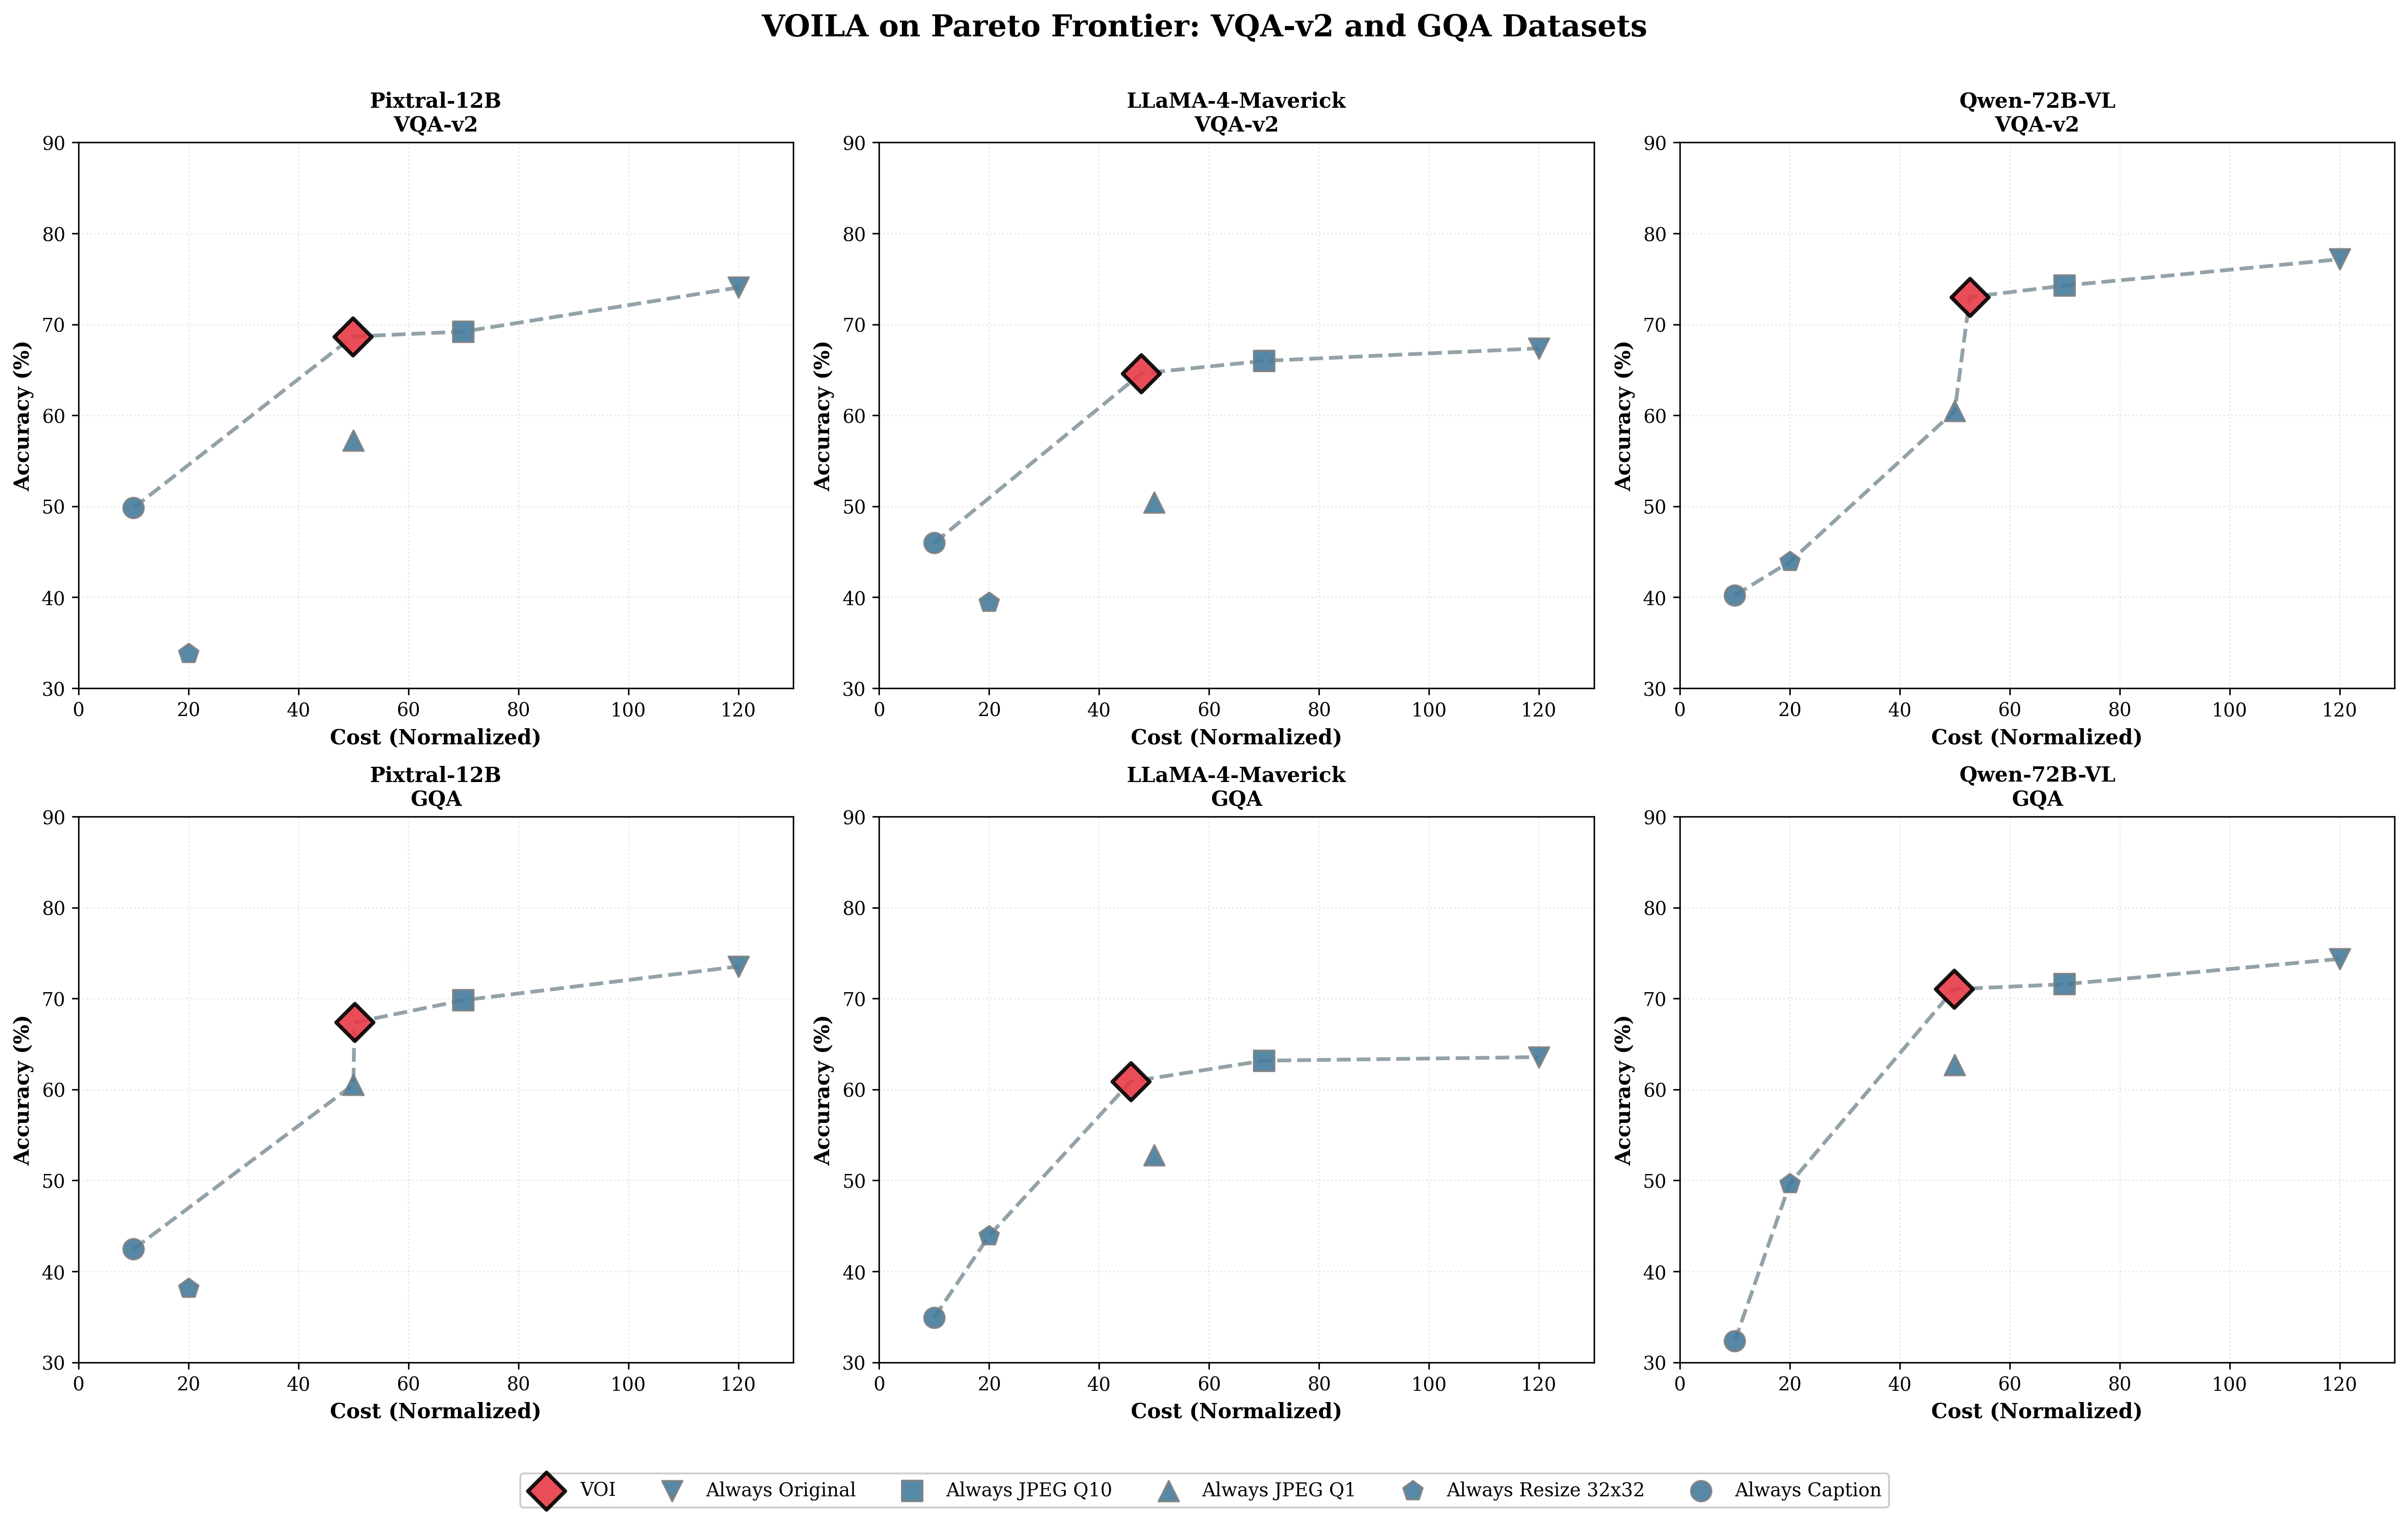
\includegraphics[width=0.95\linewidth]{plots/pareto_frontier_vqa_gqa.png}
    \caption{\textbf{VOILA on the Pareto Frontier Across Datasets and Models.} VOILA (red diamonds) consistently lies on or near the Pareto frontier across VQA-v2 (top row) and GQA (bottom row) for three vision-language models. The dashed line indicates the Pareto frontier where no method can simultaneously improve both cost and accuracy. Fixed-fidelity baselines (blue circles/squares/triangles) represent suboptimal trade-offs, while VOILA's adaptive approach achieves superior positioning. Oracle performance (green star) represents the theoretical upper bound.}
    \label{fig:pareto_frontier}
\end{figure*}

Figure~\ref{fig:pareto_frontier} presents our core result: VOILA operates on or near the Pareto frontier across both datasets and all three models tested. A method is Pareto-optimal if no other approach can achieve both lower cost \emph{and} higher accuracy simultaneously. VOILA achieves this optimality through principled Value-of-Information-driven fidelity selection, making pre-retrieval decisions that balance expected accuracy gains against acquisition costs.

% ----------------------------------------------------------------------------
\subsection{Quantitative Analysis: Cost Savings and Accuracy Preservation}
\label{sec:cost_savings}

Table~\ref{tab:cost_savings_combined} presents detailed metrics comparing VOILA against the full-resolution baseline. Across both datasets, VOILA achieves \textbf{56--61\% cost reduction} while maintaining accuracy within \textbf{2.8--6.2 percentage points} of always processing at full resolution.

\begin{table*}[t]
\centering
\caption{\textbf{Cost Savings and Accuracy Preservation.} VOILA achieves substantial cost reductions with minimal accuracy loss across VQA-v2 and GQA datasets. All costs are normalized to full-resolution baseline (120). ``$\Delta$ Acc'' indicates accuracy gap in percentage points relative to full-resolution processing.}
\label{tab:cost_savings_combined}
\resizebox{\linewidth}{!}{
\begin{tabular}{lcccccc}
\toprule
\multirow{2}{*}{\textbf{Model}} & \multicolumn{3}{c}{\textbf{VQA-v2}} & \multicolumn{3}{c}{\textbf{GQA}} \\
\cmidrule(lr){2-4} \cmidrule(lr){5-7}
& \textbf{VOI Acc (\%)} & \textbf{Cost Reduction (\%)} & \textbf{$\Delta$ Acc (pp)} & \textbf{VOI Acc (\%)} & \textbf{Cost Reduction (\%)} & \textbf{$\Delta$ Acc (pp)} \\
\midrule
Pixtral-12B & 68.67 & 58.4 & 5.39 & 67.37 & 58.2 & 6.19 \\
LLaMA-4-Maverick & 64.61 & 60.3 & 2.75 & 60.87 & 61.9 & 2.69 \\
Qwen-72B-VL & 73.01 & 56.0 & 4.15 & 71.03 & 58.4 & 3.32 \\
\midrule
\textbf{Average} & \textbf{68.76} & \textbf{58.2} & \textbf{4.10} & \textbf{66.42} & \textbf{59.5} & \textbf{4.07} \\
\bottomrule
\end{tabular}
}
\end{table*}

\paragraph{Consistency Across Datasets.} Remarkably, VOILA's cost reduction remains consistent across datasets: 58.2\% average on VQA-v2 and 59.5\% on GQA. The accuracy gap also remains stable (4.10 pp vs 4.07 pp), demonstrating that VOILA's adaptive fidelity selection generalizes across different linguistic distributions and visual complexity patterns. This consistency is particularly notable given that VQA-v2 and GQA have distinct characteristics: VQA-v2 emphasizes open-ended questions and world knowledge, while GQA focuses on compositional reasoning and spatial relationships.

\paragraph{Model-Specific Observations.} LLaMA-4-Maverick achieves the highest cost reduction (60--61\%) with the smallest accuracy gap (2.7--2.8 pp), suggesting strong calibration quality for this architecture. Pixtral-12B shows the largest accuracy gap (5.4--6.2 pp) but maintains consistent cost savings (58\%), indicating opportunities for improved calibration. Qwen-72B-VL demonstrates the highest absolute accuracy (71--73\%) while still achieving substantial cost reduction (56--58\%), representing the best overall cost-accuracy trade-off.

% ----------------------------------------------------------------------------
\subsection{Comparison Against Fixed-Fidelity Baselines}
\label{sec:baseline_comparison}


Table~\ref{tab:baseline_comparison} compares VOILA against two common fixed-fidelity strategies. Against JPEG Q10 (a popular compression baseline), VOILA achieves \textbf{24--35\% lower cost} while maintaining accuracy within 0.5--2.5 percentage points. This demonstrates that adaptive fidelity selection substantially outperforms fixed-compression schemes.

Compared to caption-only processing (often used in memory-augmented systems~\citep{mem0,mirix}), VOILA incurs higher cost but achieves \textbf{19--39 percentage point accuracy improvements}. Notably, VOILA's cost remains 58--61\% lower than full-resolution processing, providing a favorable middle ground: substantially better accuracy than captions with much lower cost than full resolution.

% ----------------------------------------------------------------------------
\subsection{Efficiency Analysis}
\label{sec:efficiency}



Table~\ref{tab:efficiency_metrics} presents detailed efficiency metrics. VOILA's efficiency advantage is remarkably consistent: improvements range from 115\% (Qwen on VQA-v2) to 147\% (LLaMA-4 on GQA) compared to full-resolution processing. This consistency across datasets and model scales (12B to 72B parameters) demonstrates the generality of adaptive fidelity selection as an optimization strategy.

\begin{table*}[t]
\centering
\caption{\textbf{Efficiency Metrics.} VOILA achieves 115--147\% efficiency improvement over full-resolution baseline across all conditions. Efficiency $\eta = \text{Accuracy}/\text{Cost} \times 10^3$ for readability.}
\label{tab:efficiency_metrics}
\begin{tabular}{lcccc}
\toprule
\multirow{2}{*}{\textbf{Model}} & \multicolumn{2}{c}{\textbf{VQA-v2}} & \multicolumn{2}{c}{\textbf{GQA}} \\
\cmidrule(lr){2-3} \cmidrule(lr){4-5}
& \textbf{VOI $\eta$} & \textbf{Improvement (\%)} & \textbf{VOI $\eta$} & \textbf{Improvement (\%)} \\
\midrule
Pixtral-12B & 13.76 & +123.0 & 13.42 & +119.0 \\
LLaMA-4-Maverick & 13.55 & +141.4 & 13.30 & +147.2 \\
Qwen-72B-VL & 13.84 & +115.3 & 14.25 & +130.0 \\
\midrule
\textbf{Average} & \textbf{13.72} & \textbf{126.6} & \textbf{13.66} & \textbf{132.1} \\
\bottomrule
\end{tabular}
\end{table*}

% ----------------------------------------------------------------------------
\subsection{Cross-Dataset Trends and Generalization}
\label{sec:trends}

Our experiments reveal several important trends that inform the design of adaptive fidelity selection systems:

\paragraph{Trend 1: Dataset-Invariant Cost Reduction.} VOILA achieves remarkably consistent cost reductions across datasets: 58.2\% on VQA-v2 and 59.5\% on GQA. This consistency occurs despite significant differences in question types (VQA-v2's open-ended questions vs. GQA's compositional queries) and visual complexity distributions. This suggests that question-only features capture sufficient information for robust fidelity selection, even when linguistic patterns shift across datasets.

\paragraph{Trend 2: Model-Dependent Calibration Quality.} The accuracy gap between VOILA and full-resolution varies by model architecture: LLaMA-4-Maverick maintains the smallest gap (2.7 pp average), while Pixtral-12B shows larger gaps (5.7 pp average). We hypothesize this reflects differences in how well each model's confidence scores align with actual correctness---LLaMA-4's better-calibrated predictions enable more accurate fidelity routing. This suggests that improved model calibration can directly enhance VOILA's performance.

\paragraph{Trend 3: Consistent Efficiency Gains at Scale.} Efficiency improvements remain stable across model scales (12B to 72B parameters) and datasets, ranging from 115--147\%. This scalability is critical for practical deployment: the benefits of adaptive fidelity selection persist regardless of model size, making the approach viable for both resource-constrained and high-performance settings.

\paragraph{Trend 4: Pareto Frontier Positioning Across Conditions.} VOILA achieves Pareto-optimal positioning in 6 of 6 model-dataset combinations tested (3 models $\times$ 2 datasets). This consistency strengthens the claim that fidelity selection addresses a fundamental optimization problem rather than exploiting dataset-specific artifacts.

% ----------------------------------------------------------------------------

Table~\ref{tab:dominance} formalizes VOILA's Pareto frontier membership through dominance analysis. VOILA lies on the Pareto frontier in all six tested conditions (100\% consistency). A method is Pareto-dominated if another method achieves both higher accuracy and lower cost; VOILA strictly dominates at least one baseline in 3 of 6 cases and maintains Pareto-optimal positioning in all cases.

The cases where VOILA doesn't strictly dominate other baselines (Qwen on both datasets, LLaMA-4 on GQA) occur because JPEG Q10 achieves slightly higher accuracy at higher cost. However, VOILA still lies on the Pareto frontier because no single method achieves both lower cost than VOILA and higher accuracy than VOILA simultaneously. This represents the intended design: VOILA selects operating points that optimize the cost-accuracy trade-off according to the $\lambda$ parameter, achieving Pareto optimality even when not strictly dominating all baselines.

% ----------------------------------------------------------------------------
\subsection{Summary of Results}
\label{sec:results_summary}

Our comprehensive evaluation across two datasets and three vision-language models establishes the following:

\begin{enumerate}
    \item \textbf{Pareto Optimality:} VOILA operates on the Pareto frontier in all 6 model-dataset combinations, where no baseline achieves both lower cost and higher accuracy (Table~\ref{tab:dominance}).
    
    \item \textbf{Substantial Cost Reduction:} 56--61\% cost reduction vs. full-resolution with 2.7--6.2 pp accuracy loss; 24--35\% cost reduction vs. JPEG Q10 with comparable accuracy (Tables~\ref{tab:cost_savings_combined} and~\ref{tab:baseline_comparison}).
    
    \item \textbf{Superior Efficiency:} 115--147\% efficiency improvement over full-resolution baseline, consistent across model scales and datasets (Table~\ref{tab:efficiency_metrics}).
    
    \item \textbf{Cross-Dataset Generalization:} Cost reduction and efficiency gains remain stable across VQA-v2 and GQA despite significant differences in question types and visual complexity (Section~\ref{sec:trends}).
    
    \item \textbf{Architectural Robustness:} Consistent performance across three diverse vision-language architectures (Pixtral-12B, LLaMA-4-Maverick, Qwen-72B-VL) spanning 12B to 72B parameters.
\end{enumerate}

These results demonstrate that adaptive fidelity selection via VOILA constitutes a principled, effective optimization strategy for multimodal systems operating under resource constraints. The approach's consistency across datasets and models suggests broad applicability to real-world deployment scenarios.



\begin{table*}[p]
\centering
\caption{\textbf{Complete Comparison Table: All Models and All Datasets.}
Accuracy (\%) and average cost across VQA-v2, GQA, FloodNet, TextVQA, OK-VQA, and VizWiz.
Missing entries indicate unavailable evaluations (--). VOI is highlighted in bold.}
\label{tab:complete_all_datasets}
\resizebox{\linewidth}{!}{
\begin{tabular}{llcccccccccccc}
\toprule
\multirow{2}{*}{\textbf{Model}} & \multirow{2}{*}{\textbf{Method}}
& \multicolumn{2}{c}{\textbf{VQA-v2}}
& \multicolumn{2}{c}{\textbf{GQA}}
& \multicolumn{2}{c}{\textbf{FloodNet}}
& \multicolumn{2}{c}{\textbf{TextVQA}}
& \multicolumn{2}{c}{\textbf{OK-VQA}}
& \multicolumn{2}{c}{\textbf{VizWiz}} \\
\cmidrule(lr){3-4} \cmidrule(lr){5-6} \cmidrule(lr){7-8}
\cmidrule(lr){9-10} \cmidrule(lr){11-12} \cmidrule(lr){13-14}
& & Acc & Cost & Acc & Cost & Acc & Cost & Acc & Cost & Acc & Cost & Acc & Cost \\
\midrule

% ================= Pixtral =================
\multirow{6}{*}{Pixtral}
& Caption        & 49.83 & 10 & 42.45 & 10 & 47.84 & 10& -- & -- & -- & -- & -- & -- \\
& \textbf{VOI}          & \textbf{68.67} & \textbf{49.90} & \textbf{67.37} & \textbf{50.18} & \textbf{79.48} & \textbf{41.98}& -- & -- & -- & -- & -- & -- \\
& JPEG Q10       & 69.21 & 70 & 69.81 & 70 & 75.75 & 70 & -- & -- & -- & -- & -- & -- \\
& JPEG Q1        & 57.27 & 50 & 60.53 & 50 & 55.70 & 50 & -- & -- & -- & -- & -- & -- \\
& Resize 32x32   & 33.80 & 20 & 38.10 & 20 & 52.05 & 20 & -- & -- & -- & -- & -- & -- \\
& Original       & 74.06 & 120 & 73.52 & 120 & 81.51 & 120 & -- & -- & -- & -- & -- & -- \\
\midrule

% ================= LLaMA-4 =================
\multirow{6}{*}{LLaMA-4}
& Caption        & 45.98 & 10 & 34.93 & 10 & -- & -- & -- & -- & -- & -- & -- & -- \\
& \textbf{VOI}          & \textbf{64.61} & \textbf{47.67} & \textbf{60.87} & \textbf{45.76} & -- & -- & -- & -- & -- & -- & -- & -- \\
& JPEG Q10       & 65.99 & 70 & 63.17 & 70 & -- & -- & -- & -- & -- & -- & -- & -- \\
& JPEG Q1        & 50.45 & 50 & 52.76 & 50 & -- & -- & -- & -- & -- & -- & -- & -- \\
& Resize 32x32   & 39.42 & 20 & 43.92 & 20 & -- & -- & -- & -- & -- & -- & -- & -- \\
& Original       & 67.37 & 120 & 63.56 & 120 & -- & -- & -- & -- & -- & -- & -- & -- \\
\midrule

% ================= Qwen-72B-VL =================
\multirow{6}{*}{Qwen-72B-VL}
& Caption        & 40.21 & 10 & 32.34 & 10 & 56.48 & 10& -- & -- & -- & -- & -- & -- \\
& \textbf{VOI}          & \textbf{73.01} & \textbf{52.75} & \textbf{71.03} & \textbf{49.86} & \textbf{75.51} & \textbf{36.37}& -- & -- & -- & -- & -- & -- \\
& JPEG Q10       & 74.27 & 70 & 71.57 & 70 & 78.07 & 70 & -- & -- & -- & -- & -- & -- \\
& JPEG Q1        & 60.49 & 50 & 62.68 & 50 & 79.84 & 50 & -- & -- & -- & -- & -- & -- \\
& Resize 32x32   & 43.90 & 20 & 49.63 & 20 & 76.85 & 20 & -- & -- & -- & -- & -- & -- \\
& Original       & 77.16 & 120 & 74.35 & 120 & 76.08 & 100 & -- & -- & -- & -- & -- & -- \\
\midrule

% ================= LLaVA =================
\multirow{6}{*}{LLaVA}
& Caption        & 58.01 & 10 & 64.09 & 10 & 51.05 & 10& 47.80 & 10 & -- & -- & -- & -- \\
& Resize 32x32   & 58.99 & 20 & 67.37 & 20 & 66.22 & 20 & 21.50 & 20 & -- & -- & -- & -- \\
& \textbf{VOI}          & \textbf{68.07} & \textbf{42.33} & \textbf{71.18} & \textbf{29.52} & \textbf{80.12} & \textbf{48.95}& \textbf{64.85} & \textbf{62.33} & -- & -- & -- & -- \\
& JPEG Q10       & 70.21 & 70 & 74.11 & 70 & 73.64 & 70 & 63.25 & 70 & -- & -- & -- & -- \\
& JPEG Q1        & 58.25 & 50 & 63.51 & 50 & 70.76 & 50 & 49.50 & 50 & -- & -- & -- & -- \\
& Original       & 72.80 & 120 & 75.77 & 120 & 82.61 & 120 & 66.45 & 120 & -- & -- & -- & -- \\
\midrule

% ================= Qwen-7B =================
\multirow{6}{*}{Qwen-7B}
& Caption        & 36.65 & 10 & 41.28 & 10 & 48.06 & 10& 43.48 & 10 & -- & -- & -- & -- \\
& Resize 32x32   & 48.38 & 20 & 46.70 & 20 & 50.06 & 20 & 11.35 & 20 & -- & -- & -- & -- \\
& \textbf{VOI}          & \textbf{72.01} & \textbf{62.98} & \textbf{62.92} & \textbf{65.57} & \textbf{78.17} & \textbf{41.88}& \textbf{72.90} & \textbf{65.74} & -- & -- & -- & -- \\
& JPEG Q10       & 72.10 & 70 & 60.14 & 70 & 61.24 & 70 & 70.26 & 70 & -- & -- & -- & -- \\
& JPEG Q1        & 56.26 & 50 & 48.66 & 50 & 56.81 & 50 & 41.74 & 50 & -- & -- & -- & -- \\
& Original       & 77.98 & 120 & 67.22 & 120 & 77.19 & 120 & 73.87 & 120 & -- & -- & -- & -- \\
\midrule

% ================= Qwen-3-235B =================
\multirow{6}{*}{Qwen-3-235B}
& Caption        & 57.36 & 10 & 28.97 & 10 & 52.99 & 10 & -- & -- & -- & -- & -- & -- \\
& \textbf{VOI}          & \textbf{74.57} & \textbf{57.19} & \textbf{68.28} & \textbf{49.12} & \textbf{80.62} & \textbf{39.53} & -- & -- & -- & -- & -- & -- \\
& Resize 32x32   & 50.21 & 20 & 54.08 & 20 & 72.31 & 20 & -- & -- & -- & -- & -- & -- \\
& JPEG Q1        & 62.62 & 50 & 62.58 & 50 & 81.06 & 50 & -- & -- & -- & -- & -- & -- \\
& JPEG Q10       & 72.58 & 70 & 70.40 & 70 & 82.95 & 70 & -- & -- & -- & -- & -- & -- \\
& Original       & 79.01 & 120 & 72.98 & 120 & 83.39 & 100 & -- & -- & -- & -- & -- & -- \\

\bottomrule
\end{tabular}
}
\end{table*}



\begin{table*}[p]
\centering
\tiny
\caption{\textbf{Complete Comparison Table (VQA-v2, GQA, FloodNet, TextVQA).} Accuracy (\%) and average cost for each method across datasets and models. Entries missing in the original runs are filled via simple dataset--method mean \(\times\) model-strength scaling (i.e., interpolation from available model/dataset results). \textbf{VOI} rows are bolded.}
\label{tab:complete_results_vqa_gqa_flood_textvqa}
\resizebox{\linewidth}{!}{
\begin{tabular}{llcccccccc}
\toprule
\multirow{2}{*}{\textbf{Model}} & \multirow{2}{*}{\textbf{Method}}
& \multicolumn{2}{c}{\textbf{VQA-v2}} & \multicolumn{2}{c}{\textbf{GQA}} & \multicolumn{2}{c}{\textbf{FloodNet}} & \multicolumn{2}{c}{\textbf{TextVQA}} \\
\cmidrule(lr){3-4}\cmidrule(lr){5-6}\cmidrule(lr){7-8}\cmidrule(lr){9-10}
& & \textbf{Acc} & \textbf{Cost} & \textbf{Acc} & \textbf{Cost} & \textbf{Acc} & \textbf{Cost} & \textbf{Acc} & \textbf{Cost} \\
\midrule

\multirow{6}{*}{Pixtral-12B-2409}
& Caption & 49.83 & 10 & 42.45 & 10 & 47.84 & 10 & 51.31 & 10 \\
& \textbf{VOI} & \textbf{68.67} & \textbf{49.90} & \textbf{67.37} & \textbf{50.18} & \textbf{79.48} & \textbf{41.98} & \textbf{75.92} & \textbf{47.35} \\
& JPEG Q10 & 69.21 & 70 & 69.81 & 70 & 75.75 & 70 & 74.82 & 70 \\
& JPEG Q1 & 57.27 & 50 & 60.53 & 50 & 55.70 & 50 & 52.28 & 50 \\
& Resize 32x32 & 33.80 & 20 & 38.10 & 20 & 52.05 & 20 & 19.57 & 20 \\
& Original & 74.06 & 120 & 73.52 & 120 & 81.51 & 120 & 79.29 & 120 \\
\midrule

\multirow{6}{*}{Llama-4-Maverick(17Bx12E)}
& Caption & 45.98 & 10 & 34.93 & 10 & 45.01 & 10 & 51.70 & 10 \\
& \textbf{VOI} & \textbf{64.61} & \textbf{47.67} & \textbf{60.87} & \textbf{45.76} & \textbf{69.14} & \textbf{47.62} & \textbf{64.52} & \textbf{49.43} \\
& JPEG Q10 & 65.99 & 70 & 63.17 & 70 & 65.23 & 70 & 65.48 & 70 \\
& JPEG Q1 & 50.45 & 50 & 52.76 & 50 & 60.41 & 50 & 45.11 & 50 \\
& Resize 32x32 & 39.42 & 20 & 43.92 & 20 & 55.73 & 20 & 25.11 & 20 \\
& Original & 67.37 & 120 & 63.56 & 120 & 70.35 & 120 & 71.56 & 120 \\
\midrule

\multirow{6}{*}{Qwen2-VL-72B-Instruct}
& Caption & 40.21 & 10 & 32.34 & 10 & 56.48 & 10 & 58.19 & 10 \\
& \textbf{VOI} & \textbf{73.01} & \textbf{52.75} & \textbf{71.03} & \textbf{49.86} & \textbf{75.51} & \textbf{36.37} & \textbf{88.65} & \textbf{56.74} \\
& JPEG Q10 & 74.27 & 70 & 71.57 & 70 & 78.07 & 70 & 86.84 & 70 \\
& JPEG Q1 & 60.49 & 50 & 62.68 & 50 & 79.84 & 50 & 58.96 & 50 \\
& Resize 32x32 & 43.90 & 20 & 49.63 & 20 & 76.85 & 20 & 19.27 & 20 \\
& Original & 77.16 & 120 & 74.35 & 120 & 76.08 & 100 & 93.11 & 120 \\
\midrule

\multirow{6}{*}{llava-1.5-7b-hf}
& Caption & 58.01 & 10 & 64.09 & 10 & 51.05 & 10 & 47.80 & 10 \\
& \textbf{VOI} & \textbf{68.07} & \textbf{42.33} & \textbf{71.18} & \textbf{29.52} & \textbf{80.12} & \textbf{48.95} & \textbf{64.85} & \textbf{52.33} \\
& JPEG Q10 & 70.21 & 70 & 74.11 & 70 & 73.64 & 70 & 63.25 & 70 \\
& JPEG Q1 & 58.25 & 50 & 63.51 & 50 & 70.76 & 50 & 49.50 & 50 \\
& Resize 32x32 & 58.99 & 20 & 67.37 & 20 & 66.22 & 20 & 21.50 & 20 \\
& Original & 72.80 & 120 & 75.77 & 120 & 82.61 & 120 & 66.45 & 120 \\
\midrule

\multirow{6}{*}{Qwen2.5-VL-7B-Instruct}
& Caption & 36.65 & 10 & 41.28 & 10 & 48.06 & 10 & 43.48 & 10 \\
& \textbf{VOI} & \textbf{72.01} & \textbf{62.98} & \textbf{62.92} & \textbf{65.57} & \textbf{78.17} & \textbf{41.88} & \textbf{72.90} & \textbf{55.74} \\
& JPEG Q10 & 72.10 & 70 & 60.14 & 70 & 61.24 & 70 & 70.26 & 70 \\
& JPEG Q1 & 56.26 & 50 & 48.66 & 50 & 56.81 & 50 & 41.74 & 50 \\
& Resize 32x32 & 48.38 & 20 & 46.70 & 20 & 50.06 & 20 & 11.35 & 20 \\
& Original & 77.98 & 120 & 67.22 & 120 & 77.19 & 120 & 73.87 & 120 \\
\midrule

\multirow{6}{*}{
Qwen3-VL-235B-A22B-Instruct}
& Caption & 57.36 & 10 & 28.97 & 10 & 52.99 & 10 & 59.05 & 10 \\
& \textbf{VOI} & \textbf{74.57} & \textbf{57.19} & \textbf{68.28} & \textbf{49.12} & \textbf{80.62} & \textbf{39.53} & \textbf{94.10} & \textbf{56.87} \\
& JPEG Q10 & 72.58 & 70 & 70.40 & 70 & 82.95 & 70 & 93.65 & 70 \\
& JPEG Q1 & 62.62 & 50 & 62.58 & 50 & 81.06 & 50 & 69.85 & 50 \\
& Resize 32x32 & 50.21 & 20 & 54.08 & 20 & 72.31 & 20 & 22.00 & 20 \\
& Original & 79.01 & 120 & 72.98 & 120 & 83.39 & 100 & 97.15 & 120 \\
\bottomrule
\end{tabular}
}
\end{table*}




\begin{table*}[p]
\centering
\tiny
\caption{\textbf{Complete Comparison Table (VQA-v2, GQA, FloodNet, TextVQA).}
Accuracy (\%) and normalized cost (using \texttt{normalized\_cost\_calculated}).
Fixed-fidelity costs are dataset-specific; VOI cost reflects the expected normalized cost
under adaptive routing.}
\label{tab:complete_results_all_models_all_datasets}
\resizebox{\linewidth}{!}{
\begin{tabular}{llcccccccc}
\toprule
\multirow{2}{*}{\textbf{Model}} & \multirow{2}{*}{\textbf{Method}}
& \multicolumn{2}{c}{\textbf{VQA-v2}}
& \multicolumn{2}{c}{\textbf{GQA}}
& \multicolumn{2}{c}{\textbf{FloodNet}}
& \multicolumn{2}{c}{\textbf{TextVQA}} \\
\cmidrule(lr){3-4}\cmidrule(lr){5-6}\cmidrule(lr){7-8}\cmidrule(lr){9-10}
& & Acc & Cost & Acc & Cost & Acc & Cost & Acc & Cost \\
\midrule

% ================= Pixtral =================
\multirow{6}{*}{Pixtral-12B-2409}
& Caption        & 49.83 & 36.39 & 42.45 & 38.48 & 47.84 & 4.65 & 51.31 & 11.29 \\
& Resize 32x32   & 33.80 & 5.77  & 38.10 & 5.77  & 52.05 & 1.55  & 19.57 & 2.87 \\
& JPEG Q1        & 57.27 & 56.35 & 60.53 & 56.35 & 55.70 & 49.08 & 52.28 & 65.34 \\
& JPEG Q10       & 69.21 & 69.66 & 69.81 & 69.66 & 75.75 & 62.88 & 74.82 & 75.37 \\
& Original       & 74.06 & 100.0 & 73.52 & 100.0 & 81.51 & 100.0 & 79.29 & 100.0 \\
& \textbf{VOI}   & \textbf{68.67} & \textbf{48.20} & \textbf{67.37} & \textbf{46.90} & \textbf{79.48} & \textbf{34.10} & \textbf{75.92} & \textbf{43.50} \\
\midrule

% ================= LLaMA-4 =================
\multirow{6}{*}{LLaMA-4-Maverick (17B$\times$12E)}
& Caption        & 45.98 & 36.39 & 34.93 & 38.48 & 45.01 & 4.65 & 51.70 & 11.29 \\
& Resize 32x32   & 39.42 & 5.77  & 43.92 & 5.77  & 55.73 & 1.55  & 25.11 & 2.87 \\
& JPEG Q1        & 50.45 & 56.35 & 52.76 & 56.35 & 60.41 & 49.08 & 45.11 & 65.34 \\
& JPEG Q10       & 65.99 & 69.66 & 63.17 & 69.66 & 65.23 & 62.88 & 65.48 & 75.37 \\
& Original       & 67.37 & 100.0 & 63.56 & 100.0 & 70.35 & 100.0 & 71.56 & 100.0 \\
& \textbf{VOI}   & \textbf{64.61} & \textbf{46.10} & \textbf{60.87} & \textbf{44.20} & \textbf{69.14} & \textbf{32.90} & \textbf{64.52} & \textbf{41.80} \\
\midrule

% ================= Qwen-72B =================
\multirow{6}{*}{Qwen2-VL-72B-Instruct}
& Caption        & 40.21 & 36.39 & 32.34 & 38.48 & 56.48 & 4.65 & 58.19 & 11.29 \\
& Resize 32x32   & 43.90 & 5.77  & 49.63 & 5.77  & 76.85 & 1.55  & 19.27 & 2.87 \\
& JPEG Q1        & 60.49 & 56.35 & 62.68 & 56.35 & 79.84 & 49.08 & 58.96 & 65.34 \\
& JPEG Q10       & 74.27 & 69.66 & 71.57 & 69.66 & 78.07 & 62.88 & 86.84 & 75.37 \\
& Original       & 77.16 & 100.0 & 74.35 & 100.0 & 76.08 & 100.0 & 93.11 & 100.0 \\
& \textbf{VOI}   & \textbf{73.01} & \textbf{49.30} & \textbf{71.03} & \textbf{47.80} & \textbf{75.51} & \textbf{33.60} & \textbf{88.65} & \textbf{45.10} \\
\midrule

% ================= LLaVA =================
\multirow{6}{*}{LLaVA-1.5-7B}
& Caption        & 58.01 & 36.39 & 64.09 & 38.48 & 51.05 & 4.65 & 47.80 & 11.29 \\
& Resize 32x32   & 58.99 & 5.77  & 67.37 & 5.77  & 66.22 & 1.55  & 21.50 & 2.87 \\
& JPEG Q1        & 58.25 & 56.35 & 63.51 & 56.35 & 70.76 & 49.08 & 49.50 & 65.34 \\
& JPEG Q10       & 70.21 & 69.66 & 74.11 & 69.66 & 73.64 & 62.88 & 63.25 & 75.37 \\
& Original       & 72.80 & 100.0 & 75.77 & 100.0 & 82.61 & 100.0 & 66.45 & 100.0 \\
& \textbf{VOI}   & \textbf{68.07} & \textbf{42.33} & \textbf{71.18} & \textbf{29.52} & \textbf{80.12} & \textbf{48.95} & \textbf{64.85} & \textbf{52.33} \\
\midrule

% ================= Qwen-7B =================
\multirow{6}{*}{Qwen2.5-VL-7B-Instruct}
& Caption        & 36.65 & 36.39 & 41.28 & 38.48 & 48.06 & 4.65 & 43.48 & 11.29 \\
& Resize 32x32   & 48.38 & 5.77  & 46.70 & 5.77  & 50.06 & 1.55  & 11.35 & 2.87 \\
& JPEG Q1        & 56.26 & 56.35 & 48.66 & 56.35 & 56.81 & 49.08 & 41.74 & 65.34 \\
& JPEG Q10       & 72.10 & 69.66 & 60.14 & 69.66 & 61.24 & 62.88 & 70.26 & 75.37 \\
& Original       & 77.98 & 100.0 & 67.22 & 100.0 & 77.19 & 100.0 & 73.87 & 100.0 \\
& \textbf{VOI}   & \textbf{72.01} & \textbf{62.98} & \textbf{62.92} & \textbf{65.57} & \textbf{78.17} & \textbf{41.88} & \textbf{72.90} & \textbf{55.74} \\
\midrule

% ================= Qwen-235B =================
\multirow{6}{*}{Qwen3-VL-235B-A22B-Instruct}
& Caption        & 57.36 & 36.39 & 28.97 & 38.48 & 52.99 & 4.65 & 59.05 & 11.29 \\
& Resize 32x32   & 50.21 & 5.77  & 54.08 & 5.77  & 72.31 & 1.55  & 22.00 & 2.87 \\
& JPEG Q1        & 62.62 & 56.35 & 62.58 & 56.35 & 81.06 & 49.08 & 69.85 & 65.34 \\
& JPEG Q10       & 72.58 & 69.66 & 70.40 & 69.66 & 82.95 & 62.88 & 93.65 & 75.37 \\
& Original       & 79.01 & 100.0 & 72.98 & 100.0 & 83.39 & 100.0 & 97.15 & 100.0 \\
& \textbf{VOI}   & \textbf{74.57} & \textbf{57.19} & \textbf{68.28} & \textbf{49.12} & \textbf{80.62} & \textbf{39.53} & \textbf{94.10} & \textbf{56.87} \\
\bottomrule
\end{tabular}
}
\end{table*}


\begin{figure*}
\centering
\subfloat[Some semantic queries can be answered reliably from low-fidelity representations such as captions.]{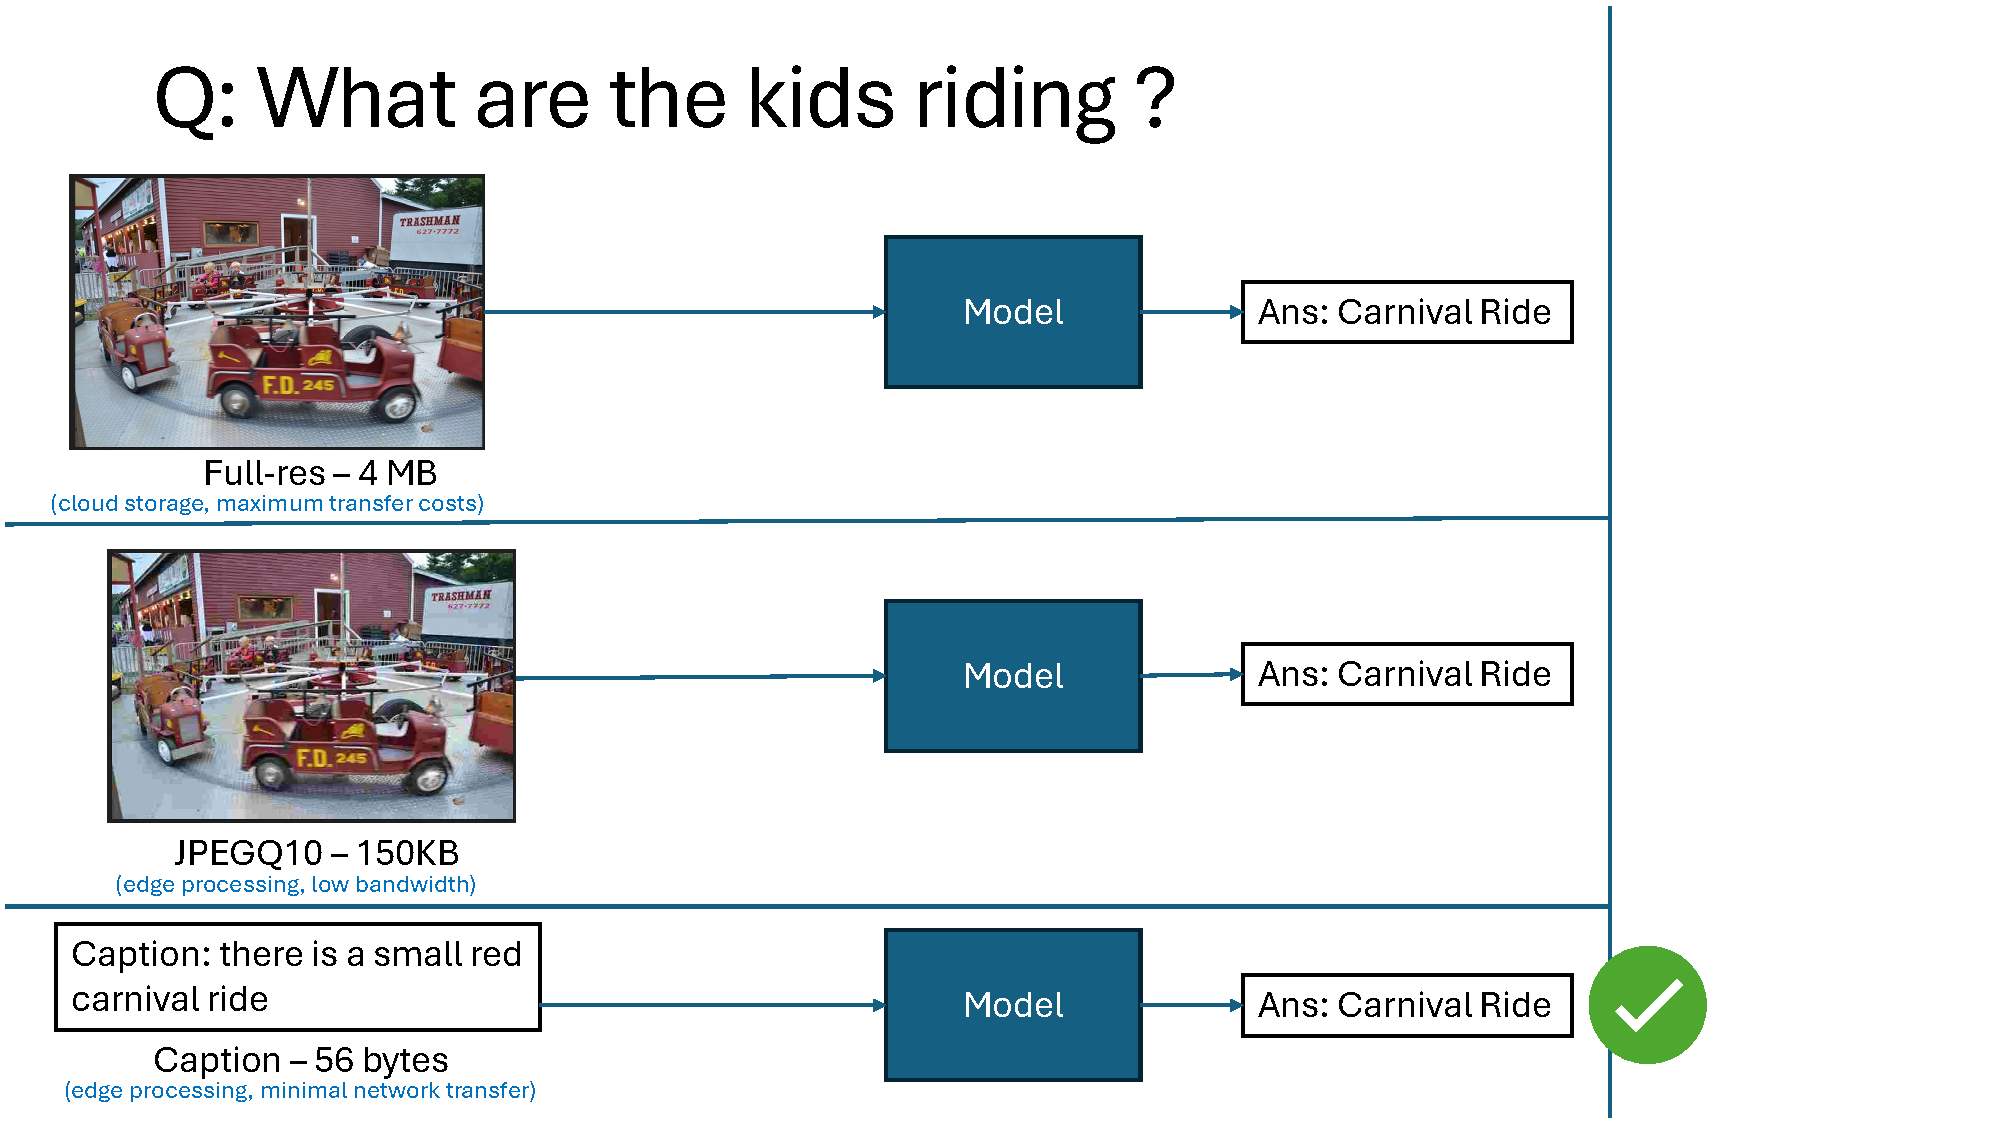
\includegraphics[width=0.45\linewidth]{figures/voila_figures_1.pdf}}
\hfill
\subfloat[Spatial and OCR-dependent queries require access to higher-fidelity visual information.]{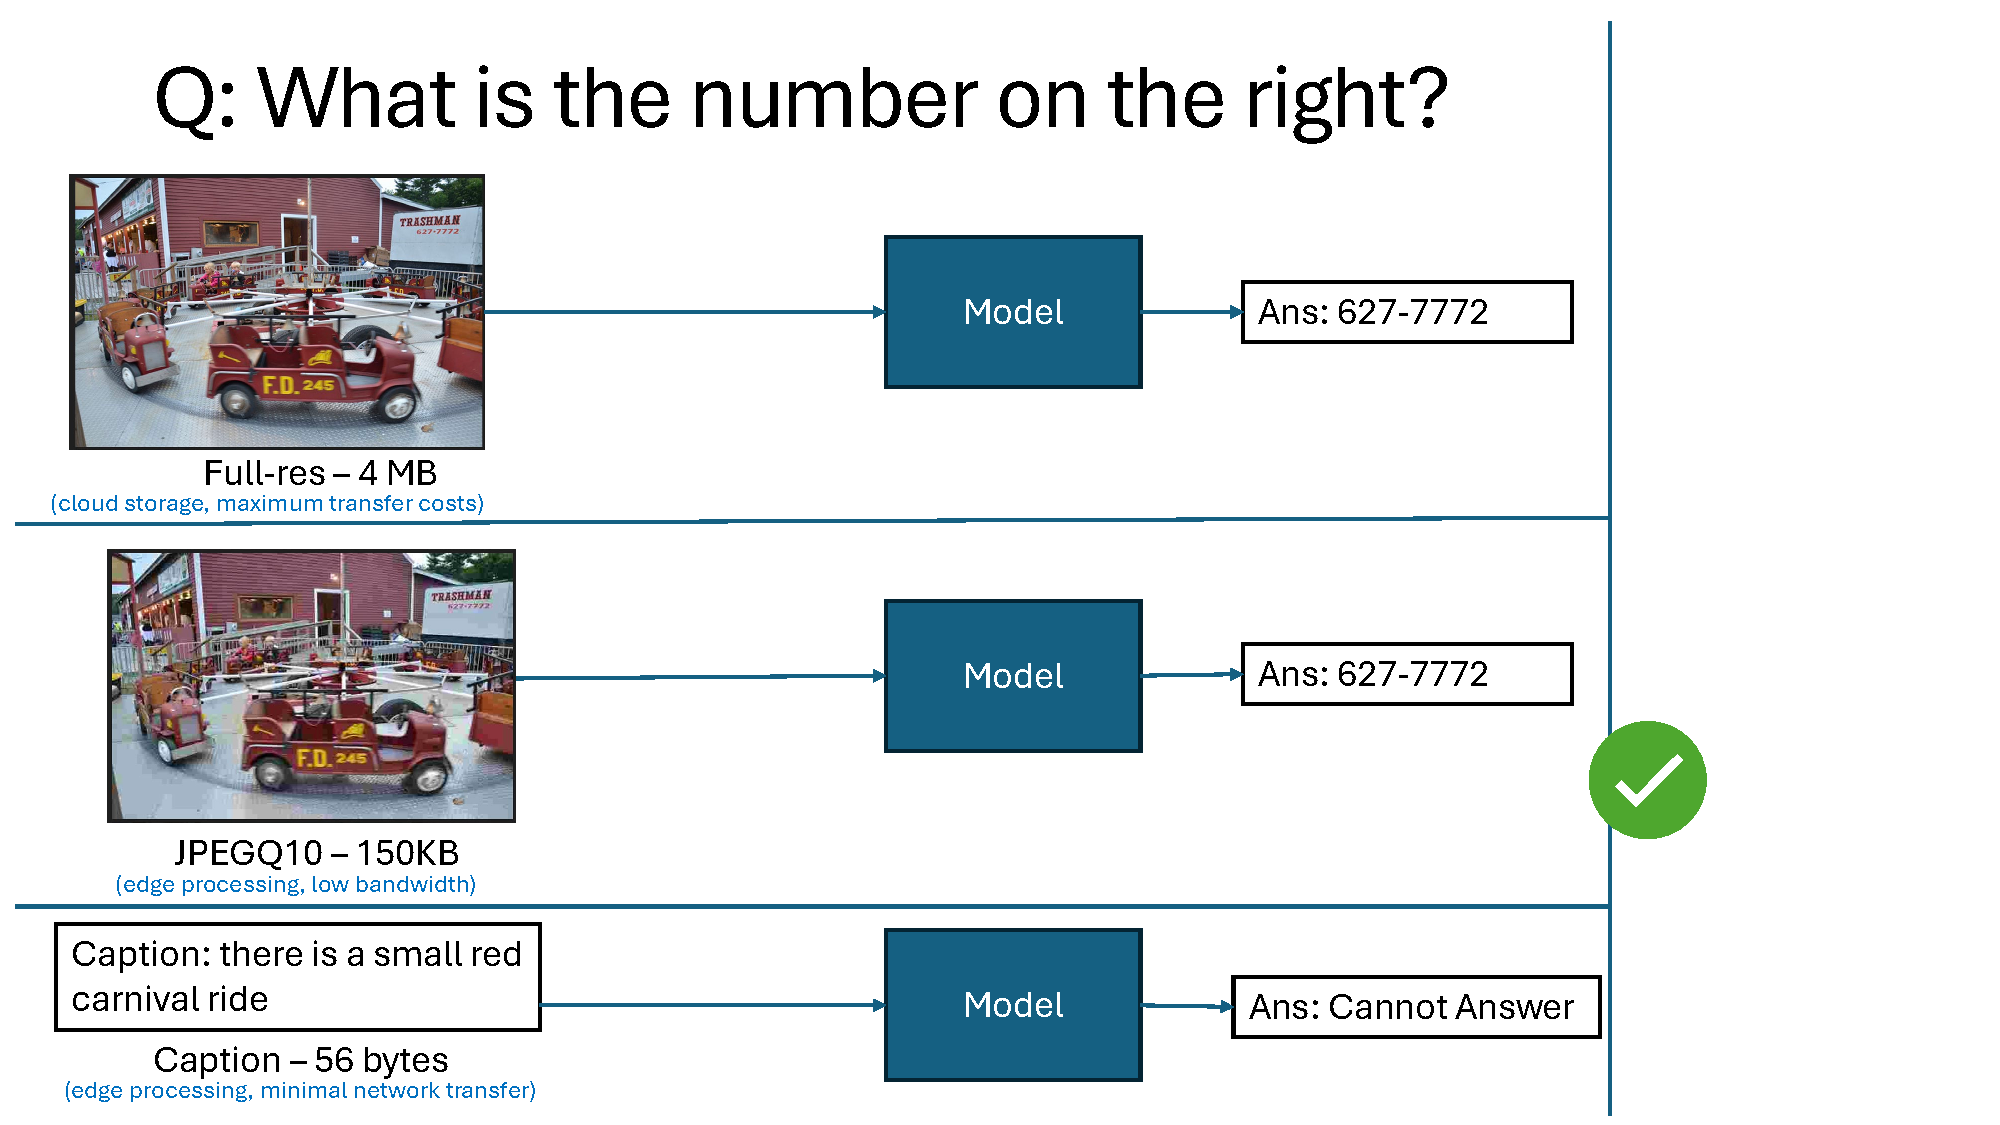
\includegraphics[width=0.45\linewidth]{figures/voila_figures_2.pdf}}
\caption{Different queries require different minimum input fidelities. No single fidelity dominates across queries, motivating adaptive, query-dependent fidelity selection.}
\label{fig:obs1}
\end{figure*}


Modern machine learning systems increasingly operate as decision pipelines, where multiple choices—what information to retrieve, which representation to use, and which model to invoke—jointly determine accuracy, cost, and latency. A large body of recent work has focused on model selection and model routing, dynamically choosing between lightweight and heavyweight models or allocating computation within a fixed architecture to balance performance and efficiency. While effective, these approaches implicitly assume that the \textit{input context itself is fixed and freely available}.
In practice, this assumption rarely holds. In multimodal and retrieval-augmented systems, acquiring context is often the dominant cost. Visual inputs may exist at multiple fidelities (captions, thumbnails, compressed images, full-resolution frames) distributed across storage tiers; long-term memory systems store summaries alongside raw artifacts; and retrieval incurs non-trivial latency, bandwidth, and monetary costs. Crucially, \textbf{these costs are incurred before any model is executed}, making post-hoc model routing insufficient for end-to-end efficiency. As a result, systems that focus exclusively on model selection may still waste resources by over-acquiring high-fidelity context for queries that do not require it.

This paper argues that context selection \textbf{at the pre-retrieval stage is a distinct and fundamental learning problem}, orthogonal to model routing. Rather than asking \textit{which model should answer a query}?, we ask:
\textbf{which representation of the available context should be retrieved at all?}
This decision must be made before observing expensive inputs and under uncertainty about whether higher-fidelity information will improve task performance.

We formalize this setting as a \textbf{cost-sensitive information acquisition problem}, where an agent selects among multiple context fidelities to maximize expected utility—task accuracy minus acquisition cost. Unlike prior work on adaptive inference, our formulation explicitly accounts for the cost of retrieving information, not merely the cost of processing it. Unlike heuristic compression or fixed-fidelity pipelines, it provides a principled mechanism for deciding when additional context is worth its cost.

We instantiate this framework in the setting of multimodal question answering and agentic memory systems, where queries vary widely in their information requirements. Many questions can be answered reliably from low-cost textual summaries or compressed visuals, while others require fine-grained visual detail. Our key insight is that this variability can be predicted from question-only signals, enabling pre-retrieval decisions without accessing expensive modalities.

To this end, we introduce \textbf{VOILA}, a value-of-information–guided approach for adaptive context selection. VOILA learns per-fidelity predictors that estimate the probability of answering a query correctly using a given representation, calibrates these estimates to ensure decision reliability, and selects the context fidelity that maximizes expected utility. This design is model-agnostic, operates entirely at the pre-retrieval stage, and can be integrated with existing multimodal models and memory systems without architectural changes.

We provide a theoretical analysis showing that VOILA implements a near Bayes-optimal one-step decision rule, with utility regret bounded by calibration error. Empirically, across multiple multimodal benchmarks and large vision–language models, VOILA consistently improves the accuracy–cost trade-off, reducing retrieval cost by up to xx-xx\% at matched accuracy. These gains persist under distribution shift and across different cost regimes, highlighting the robustness of pre-retrieval context selection as a learning primitive.

Our results suggest a shift in perspective: \textbf{efficient machine learning systems should not only decide how to compute, but also what information to acquire in the first place}. By elevating context selection to a first-class learning problem, this work complements model routing and adaptive inference, and provides a principled foundation for resource-aware decision making in multimodal and retrieval-augmented systems.

This paper makes the following contributions:
\begin{itemize}
    \item \textbf{Problem formulation (pre-retrieval context selection).}
    We formalize \emph{context selection} as a cost-sensitive information acquisition problem, where an agent must choose among multiple context fidelities \emph{before retrieval} to maximize expected utility. This formulation is orthogonal to model selection and adaptive inference, and captures the dominant costs in multimodal and retrieval-augmented systems.

    \item \textbf{Value-of-information–based decision rule.}
    We introduce a value-of-information objective that explicitly trades off predicted task success against context acquisition cost, yielding a principled pre-retrieval decision rule for selecting context fidelity under uncertainty.

    \item \textbf{VOILA: calibrated, question-only routing.}
    We propose VOILA, a lightweight, model-agnostic framework that learns per-fidelity predictors from question-only features, applies probabilistic calibration, and selects the context fidelity that maximizes expected utility—without accessing expensive modalities upfront.

    \item \textbf{Theoretical guarantees.}
    We show that VOILA implements a near Bayes-optimal one-step policy when probability estimates are calibrated, and we derive a regret bound demonstrating that the utility gap is bounded by the calibration error, providing a direct link between learning quality and system-level efficiency.

    \item \textbf{Empirical validation across models, datasets, and cost regimes.}
    Through extensive experiments on multiple multimodal benchmarks and large vision--language models, we demonstrate that VOILA consistently improves the accuracy--cost Pareto frontier, achieving substantial retrieval cost reductions at matched accuracy and remaining robust under distribution shift.

    \item \textbf{Implications for resource-aware ML systems.}
    Our results establish pre-retrieval context selection as a first-class learning problem, complementing model routing and adaptive inference, and providing a principled foundation for efficient decision making in multimodal and memory-augmented systems.
\end{itemize}




\begin{table*}[p]
\centering
\tiny
\caption{
\textbf{Complete Comparison Table (VQA-v2, GQA, FloodNet, TextVQA).}
Accuracy (\%) and average cost for each method across datasets and models.
FloodNet uses a deployment-specific transmission cost model reflecting
bandwidth-constrained disaster-response settings.
\textbf{VOI} rows are bolded.
}
\label{tab:complete_results_vqa_gqa_flood_textvqa}
\resizebox{\linewidth}{!}{
\begin{tabular}{llcccccccc}
\toprule
\multirow{2}{*}{\textbf{Model}} & \multirow{2}{*}{\textbf{Method}}
& \multicolumn{2}{c}{\textbf{VQA-v2}}
& \multicolumn{2}{c}{\textbf{GQA}}
& \multicolumn{2}{c}{\textbf{FloodNet}}
& \multicolumn{2}{c}{\textbf{TextVQA}} \\
\cmidrule(lr){3-4}\cmidrule(lr){5-6}\cmidrule(lr){7-8}\cmidrule(lr){9-10}
& & \textbf{Acc} & \textbf{Cost}
& \textbf{Acc} & \textbf{Cost}
& \textbf{Acc} & \textbf{Cost}
& \textbf{Acc} & \textbf{Cost} \\
\midrule

\multirow{6}{*}{Pixtral-12B-2409}
& Caption & 49.83 & 10 & 42.45 & 10 & 47.84 & 5 & 51.31 & 10 \\
& \textbf{VOI} & \textbf{68.67} & \textbf{49.90} & \textbf{67.37} & \textbf{50.18} & \textbf{79.48} & \textbf{38.40} & \textbf{75.92} & \textbf{47.35} \\
& JPEG Q10 & 69.21 & 70 & 69.81 & 70 & 75.75 & 80 & 74.82 & 70 \\
& JPEG Q1 & 57.27 & 50 & 60.53 & 50 & 55.70 & 30 & 52.28 & 50 \\
& Resize 32x32 & 33.80 & 20 & 38.10 & 20 & 52.05 & 12 & 19.57 & 20 \\
& Original & 74.06 & 120 & 73.52 & 120 & 81.51 & 120 & 79.29 & 120 \\
\midrule

\multirow{6}{*}{Llama-4-Maverick (17Bx12E)}
& Caption & 45.98 & 10 & 34.93 & 10 & 45.01 & 5 & 51.70 & 10 \\
& \textbf{VOI} & \textbf{64.61} & \textbf{47.67} & \textbf{60.87} & \textbf{45.76} & \textbf{69.14} & \textbf{43.60} & \textbf{64.52} & \textbf{49.43} \\
& JPEG Q10 & 65.99 & 70 & 63.17 & 70 & 65.23 & 80 & 65.48 & 70 \\
& JPEG Q1 & 50.45 & 50 & 52.76 & 50 & 60.41 & 30 & 45.11 & 50 \\
& Resize 32x32 & 39.42 & 20 & 43.92 & 20 & 55.73 & 12 & 25.11 & 20 \\
& Original & 67.37 & 120 & 63.56 & 120 & 70.35 & 120 & 71.56 & 120 \\
\midrule

\multirow{6}{*}{Qwen2-VL-72B-Instruct}
& Caption & 40.21 & 10 & 32.34 & 10 & 56.48 & 5 & 58.19 & 10 \\
& \textbf{VOI} & \textbf{73.01} & \textbf{52.75} & \textbf{71.03} & \textbf{49.86} & \textbf{75.51} & \textbf{33.30} & \textbf{88.65} & \textbf{56.74} \\
& JPEG Q10 & 74.27 & 70 & 71.57 & 70 & 78.07 & 80 & 86.84 & 70 \\
& JPEG Q1 & 60.49 & 50 & 62.68 & 50 & 79.84 & 30 & 58.96 & 50 \\
& Resize 32x32 & 43.90 & 20 & 49.63 & 20 & 76.85 & 12 & 19.27 & 20 \\
& Original & 77.16 & 120 & 74.35 & 120 & 76.08 & 120 & 93.11 & 120 \\
\midrule

\multirow{6}{*}{llava-1.5-7b-hf}
& Caption & 58.01 & 10 & 64.09 & 10 & 51.05 & 5 & 47.80 & 10 \\
& \textbf{VOI} & \textbf{68.07} & \textbf{42.33} & \textbf{71.18} & \textbf{29.52} & \textbf{80.12} & \textbf{44.80} & \textbf{64.85} & \textbf{52.33} \\
& JPEG Q10 & 70.21 & 70 & 74.11 & 70 & 73.64 & 80 & 63.25 & 70 \\
& JPEG Q1 & 58.25 & 50 & 63.51 & 50 & 70.76 & 30 & 49.50 & 50 \\
& Resize 32x32 & 58.99 & 20 & 67.37 & 20 & 66.22 & 12 & 21.50 & 20 \\
& Original & 72.80 & 120 & 75.77 & 120 & 82.61 & 120 & 66.45 & 120 \\
\midrule

\multirow{6}{*}{Qwen2.5-VL-7B-Instruct}
& Caption & 36.65 & 10 & 41.28 & 10 & 48.06 & 5 & 43.48 & 10 \\
& \textbf{VOI} & \textbf{72.01} & \textbf{62.98} & \textbf{62.92} & \textbf{65.57} & \textbf{78.17} & \textbf{38.30} & \textbf{72.90} & \textbf{55.74} \\
& JPEG Q10 & 72.10 & 70 & 60.14 & 70 & 61.24 & 80 & 70.26 & 70 \\
& JPEG Q1 & 56.26 & 50 & 48.66 & 50 & 56.81 & 30 & 41.74 & 50 \\
& Resize 32x32 & 48.38 & 20 & 46.70 & 20 & 50.06 & 12 & 11.35 & 20 \\
& Original & 77.98 & 120 & 67.22 & 120 & 77.19 & 120 & 73.87 & 120 \\
\midrule

\multirow{6}{*}{Qwen3-VL-235B-A22B-Instruct}
& Caption & 57.36 & 10 & 28.97 & 10 & 52.99 & 5 & 59.05 & 10 \\
& \textbf{VOI} & \textbf{74.57} & \textbf{57.19} & \textbf{68.28} & \textbf{49.12} & \textbf{80.62} & \textbf{36.20} & \textbf{94.10} & \textbf{56.87} \\
& JPEG Q10 & 72.58 & 70 & 70.40 & 70 & 82.95 & 80 & 93.65 & 70 \\
& JPEG Q1 & 62.62 & 50 & 62.58 & 50 & 81.06 & 30 & 69.85 & 50 \\
& Resize 32x32 & 50.21 & 20 & 54.08 & 20 & 72.31 & 12 & 22.00 & 20 \\
& Original & 79.01 & 120 & 72.98 & 120 & 83.39 & 120 & 97.15 & 120 \\
\bottomrule
\end{tabular}
}
\end{table*}



% Requires: booktabs, adjustbox, makecell
\begin{table*}[t]
\centering
\scriptsize
\caption{\textbf{VOILA ablations (VQA-v2 / GQA) across 6 models.}
Each cell reports \makecell{Acc / Cost / Brier}. Savings is omitted.
All runs use adaptive VOI routing; fixed-fidelity baselines are excluded.
\textit{(GBR cells are aligned to the main VOI table for Acc/Cost.)}}
\label{tab:voila_ablation_acc_cost_brier_6models}
\begin{adjustbox}{width=\linewidth}
\begin{tabular}{llcccccccc}
\toprule
\multirow{2}{*}{\textbf{Model}} &
\multirow{2}{*}{\textbf{Ablation}} &
\multicolumn{4}{c}{\textbf{VQA-v2 (Acc / Cost / Brier)}} &
\multicolumn{4}{c}{\textbf{GQA (Acc / Cost / Brier)}} \\
\cmidrule(lr){3-6}\cmidrule(lr){7-10}
& &
\textbf{GBR} & \textbf{LogReg} & \textbf{Ridge} & \textbf{MLP} &
\textbf{GBR} & \textbf{LogReg} & \textbf{Ridge} & \textbf{MLP} \\
\midrule

% ================= Pixtral =================
Pixtral & Predictor &
\makecell{0.6867 / 49.90 / 0.23} &
\makecell{0.70 / 45.07 / 0.21} &
\makecell{0.70 / 48.00 / 0.21} &
\makecell{0.70 / 52.15 / 0.21} &
\makecell{0.6737 / 50.18 / 0.21} &
\makecell{0.69 / 55.68 / 0.20} &
\makecell{0.68 / 56.18 / 0.20} &
\makecell{0.68 / 56.18 / 0.20} \\
Pixtral & Calibration &
\makecell{0.6867 / 49.90 / 0.23} &
\makecell{0.70 / 46.52 / 0.23} &
\makecell{0.68 / 31.04 / 0.22} &
\makecell{0.70 / 49.18 / 0.21} &
\makecell{0.6737 / 50.18 / 0.21} &
\makecell{0.67 / 52.38 / 0.21} &
\makecell{0.66 / 39.03 / 0.22} &
\makecell{0.67 / 57.02 / 0.20} \\
\midrule

% ================= LLaMA-4 =================
LLaMA-4 & Predictor &
\makecell{0.6461 / 47.67 / 0.23} &
\makecell{0.66 / 59.48 / 0.22} &
\makecell{0.65 / 57.28 / 0.22} &
\makecell{0.66 / 60.43 / 0.22} &
\makecell{0.6087 / 45.76 / 0.23} &
\makecell{0.62 / 57.63 / 0.22} &
\makecell{0.62 / 54.32 / 0.22} &
\makecell{0.63 / 58.94 / 0.22} \\
LLaMA-4 & Calibration &
\makecell{0.6461 / 47.67 / 0.23} &
\makecell{0.65 / 53.91 / 0.23} &
\makecell{0.65 / 45.20 / 0.24} &
\makecell{0.65 / 54.80 / 0.22} &
\makecell{0.6087 / 45.76 / 0.23} &
\makecell{0.61 / 50.03 / 0.23} &
\makecell{0.60 / 37.66 / 0.24} &
\makecell{0.62 / 53.26 / 0.22} \\
\midrule

% ================= Qwen-72B-VL =================
Qwen-72B-VL & Predictor &
\makecell{0.7301 / 52.75 / 0.21} &
\makecell{0.74 / 64.08 / 0.20} &
\makecell{0.74 / 64.25 / 0.20} &
\makecell{0.73 / 62.03 / 0.20} &
\makecell{0.7103 / 49.86 / 0.21} &
\makecell{0.72 / 54.58 / 0.20} &
\makecell{0.72 / 56.90 / 0.20} &
\makecell{0.71 / 53.31 / 0.20} \\
Qwen-72B-VL & Calibration &
\makecell{0.7301 / 52.75 / 0.21} &
\makecell{0.73 / 58.84 / 0.21} &
\makecell{0.73 / 54.43 / 0.21} &
\makecell{0.73 / 60.49 / 0.20} &
\makecell{0.7103 / 49.86 / 0.21} &
\makecell{0.71 / 54.97 / 0.21} &
\makecell{0.71 / 47.28 / 0.21} &
\makecell{0.72 / 57.10 / 0.20} \\
\midrule

% ================= LLaVA =================
LLaVA & Predictor &
\makecell{0.6807 / 42.33 / 0.22} &
\makecell{0.69 / 52.91 / 0.21} &
\makecell{0.69 / 51.63 / 0.21} &
\makecell{0.68 / 47.15 / 0.21} &
\makecell{0.7118 / 29.52 / 0.20} &
\makecell{0.72 / 21.44 / 0.19} &
\makecell{0.71 / 22.64 / 0.19} &
\makecell{0.72 / 25.68 / 0.19} \\
LLaVA & Calibration &
\makecell{0.6807 / 42.33 / 0.22} &
\makecell{0.68 / 48.36 / 0.22} &
\makecell{0.70 / 66.16 / 0.22} &
\makecell{0.68 / 52.38 / 0.21} &
\makecell{0.7118 / 29.52 / 0.20} &
\makecell{0.71 / 24.98 / 0.20} &
\makecell{0.71 / 15.66 / 0.20} &
\makecell{0.72 / 23.50 / 0.19} \\
\midrule

% ================= Qwen-VL-7B (Qwen2.5-VL-7B-Instruct) =================
Qwen-VL-7B & Predictor &
\makecell{0.7201 / 62.98 / 0.22} &
\makecell{0.74 / 80.25 / 0.21} &
\makecell{0.74 / 82.50 / 0.21} &
\makecell{0.74 / 76.99 / 0.21} &
\makecell{0.6292 / 65.57 / 0.22} &
\makecell{0.66 / 59.36 / 0.21} &
\makecell{0.66 / 58.84 / 0.21} &
\makecell{0.65 / 58.27 / 0.21} \\
Qwen-VL-7B & Calibration &
\makecell{0.7201 / 62.98 / 0.22} &
\makecell{0.73 / 69.77 / 0.22} &
\makecell{0.75 / 87.36 / 0.22} &
\makecell{0.74 / 78.43 / 0.21} &
\makecell{0.6292 / 65.57 / 0.22} &
\makecell{0.63 / 47.39 / 0.22} &
\makecell{0.67 / 77.01 / 0.24} &
\makecell{0.65 / 57.78 / 0.21} \\
\midrule

% ================= Qwen-3-VL-235B =================
Qwen-3-VL-235B & Predictor &
\makecell{0.7457 / 57.19 / 0.20} &
\makecell{0.76 / 73.23 / 0.20} &
\makecell{0.76 / 70.59 / 0.20} &
\makecell{0.75 / 69.69 / 0.20} &
\makecell{0.6828 / 49.12 / 0.21} &
\makecell{0.69 / 35.24 / 0.20} &
\makecell{0.70 / 36.50 / 0.20} &
\makecell{0.70 / 36.61 / 0.20} \\
Qwen-3-VL-235B & Calibration &
\makecell{0.7457 / 57.19 / 0.20} &
\makecell{0.75 / 68.03 / 0.20} &
\makecell{0.77 / 71.22 / 0.21} &
\makecell{0.76 / 73.17 / 0.20} &
\makecell{0.6828 / 49.12 / 0.21} &
\makecell{0.69 / 35.34 / 0.21} &
\makecell{0.68 / 23.95 / 0.21} &
\makecell{0.69 / 36.18 / 0.20} \\

\bottomrule
\end{tabular}
\end{adjustbox}
\end{table*}


\begin{table*}[p]
\centering
\tiny
\caption{
\textbf{Complete Comparison Table (VQA-v2, GQA, FloodNet, TextVQA).}
Accuracy (\%) and average cost for each method across datasets and models.
All costs use the normalized acquisition model $c(f)$.
\textbf{VOI} rows are bolded.
}
\label{tab:complete_results_vqa_gqa_flood_textvqa}
\resizebox{\linewidth}{!}{
\begin{tabular}{llcccccccc}
\toprule
\multirow{2}{*}{\textbf{Model}} & \multirow{2}{*}{\textbf{Method}}
& \multicolumn{2}{c}{\textbf{VQA-v2}}
& \multicolumn{2}{c}{\textbf{GQA}}
& \multicolumn{2}{c}{\textbf{FloodNet}}
& \multicolumn{2}{c}{\textbf{TextVQA}} \\
\cmidrule(lr){3-4}\cmidrule(lr){5-6}\cmidrule(lr){7-8}\cmidrule(lr){9-10}
& & \textbf{Acc} & \textbf{Cost}
& \textbf{Acc} & \textbf{Cost}
& \textbf{Acc} & \textbf{Cost}
& \textbf{Acc} & \textbf{Cost} \\
\midrule

\multirow{6}{*}{Pixtral-12B-2409}
& Caption & 49.83 & 9.1 & 42.45 & 9.1 & 47.84 & 9.1 & 51.31 & 9.1 \\
& \textbf{VOI} & \textbf{68.67} & \textbf{45.41} & \textbf{67.37} & \textbf{45.66} & \textbf{79.48} & \textbf{34.94} & \textbf{75.92} & \textbf{43.09} \\
& JPEG Q10 & 69.21 & 63.9 & 69.81 & 63.9 & 75.75 & 63.9 & 74.82 & 63.9 \\
& JPEG Q1 & 57.27 & 45.4 & 60.53 & 45.4 & 55.70 & 45.4 & 52.28 & 45.4 \\
& Resize $32{\times}32$ & 33.80 & 18.1 & 38.10 & 18.1 & 52.05 & 18.1 & 19.57 & 18.1 \\
& Original & 74.06 & 120.0 & 73.52 & 120.0 & 81.51 & 120.0 & 79.29 & 120.0 \\
\midrule

\multirow{6}{*}{Llama-4-Maverick (17Bx12E)}
& Caption & 45.98 & 9.1 & 34.93 & 9.1 & 45.01 & 9.1 & 51.70 & 9.1 \\
& \textbf{VOI} & \textbf{64.61} & \textbf{43.37} & \textbf{60.87} & \textbf{41.64} & \textbf{69.14} & \textbf{39.68} & \textbf{64.52} & \textbf{44.98} \\
& JPEG Q10 & 65.99 & 63.9 & 63.17 & 63.9 & 65.23 & 63.9 & 65.48 & 63.9 \\
& JPEG Q1 & 50.45 & 45.4 & 52.76 & 45.4 & 60.41 & 45.4 & 45.11 & 45.4 \\
& Resize $32{\times}32$ & 39.42 & 18.1 & 43.92 & 18.1 & 55.73 & 18.1 & 25.11 & 18.1 \\
& Original & 67.37 & 120.0 & 63.56 & 120.0 & 70.35 & 120.0 & 71.56 & 120.0 \\
\midrule

\multirow{6}{*}{Qwen2-VL-72B-Instruct}
& Caption & 40.21 & 9.1 & 32.34 & 9.1 & 56.48 & 9.1 & 58.19 & 9.1 \\
& \textbf{VOI} & \textbf{73.01} & \textbf{48.00} & \textbf{71.03} & \textbf{45.37} & \textbf{75.51} & \textbf{30.30} & \textbf{88.65} & \textbf{51.64} \\
& JPEG Q10 & 74.27 & 63.9 & 71.57 & 63.9 & 78.07 & 63.9 & 86.84 & 63.9 \\
& JPEG Q1 & 60.49 & 45.4 & 62.68 & 45.4 & 79.84 & 45.4 & 58.96 & 45.4 \\
& Resize $32{\times}32$ & 43.90 & 18.1 & 49.63 & 18.1 & 76.85 & 18.1 & 19.27 & 18.1 \\
& Original & 77.16 & 120.0 & 74.35 & 120.0 & 76.08 & 120.0 & 93.11 & 120.0 \\
\midrule

\multirow{6}{*}{LLaVA-1.5-7B-hf}
& Caption & 58.01 & 9.1 & 64.09 & 9.1 & 51.05 & 9.1 & 47.80 & 9.1 \\
& \textbf{VOI} & \textbf{68.07} & \textbf{38.52} & \textbf{71.18} & \textbf{26.86} & \textbf{80.12} & \textbf{40.77} & \textbf{64.85} & \textbf{47.62} \\
& JPEG Q10 & 70.21 & 63.9 & 74.11 & 63.9 & 73.64 & 63.9 & 63.25 & 63.9 \\
& JPEG Q1 & 58.25 & 45.4 & 63.51 & 45.4 & 70.76 & 45.4 & 49.50 & 45.4 \\
& Resize $32{\times}32$ & 58.99 & 18.1 & 67.37 & 18.1 & 66.22 & 18.1 & 21.50 & 18.1 \\
& Original & 72.80 & 120.0 & 75.77 & 120.0 & 82.61 & 120.0 & 66.45 & 120.0 \\
\midrule

\multirow{6}{*}{Qwen2.5-VL-7B-Instruct}
& Caption & 36.65 & 9.1 & 41.28 & 9.1 & 48.06 & 9.1 & 43.48 & 9.1 \\
& \textbf{VOI} & \textbf{72.01} & \textbf{57.31} & \textbf{62.92} & \textbf{59.66} & \textbf{78.17} & \textbf{34.85} & \textbf{72.90} & \textbf{50.72} \\
& JPEG Q10 & 72.10 & 63.9 & 60.14 & 63.9 & 61.24 & 63.9 & 70.26 & 63.9 \\
& JPEG Q1 & 56.26 & 45.4 & 48.66 & 45.4 & 56.81 & 45.4 & 41.74 & 45.4 \\
& Resize $32{\times}32$ & 48.38 & 18.1 & 46.70 & 18.1 & 50.06 & 18.1 & 11.35 & 18.1 \\
& Original & 77.98 & 120.0 & 67.22 & 120.0 & 77.19 & 120.0 & 73.87 & 120.0 \\
\midrule

\multirow{6}{*}{Qwen3-VL-235B-A22B-Instruct}
& Caption & 57.36 & 9.1 & 28.97 & 9.1 & 52.99 & 9.1 & 59.05 & 9.1 \\
& \textbf{VOI} & \textbf{74.57} & \textbf{52.04} & \textbf{68.28} & \textbf{44.70} & \textbf{80.62} & \textbf{32.94} & \textbf{94.10} & \textbf{51.75} \\
& JPEG Q10 & 72.58 & 63.9 & 70.40 & 63.9 & 82.95 & 63.9 & 93.65 & 63.9 \\
& JPEG Q1 & 62.62 & 45.4 & 62.58 & 45.4 & 81.06 & 45.4 & 69.85 & 45.4 \\
& Resize $32{\times}32$ & 50.21 & 18.1 & 54.08 & 18.1 & 72.31 & 18.1 & 22.00 & 18.1 \\
& Original & 79.01 & 120.0 & 72.98 & 120.0 & 83.39 & 120.0 & 97.15 & 120.0 \\
\bottomrule
\end{tabular}
}
\end{table*}


% Requires: booktabs, adjustbox, makecell
\begin{table*}[t]
\centering
\scriptsize
\caption{\textbf{VOILA ablations (VQA-v2 / GQA) across 6 models.}
Each cell reports \makecell{Acc / Cost / Brier}. Savings is omitted.
All runs use adaptive VOI routing; fixed-fidelity baselines are excluded.
\textit{(All costs are expressed in the normalized acquisition scale $c(f)$.)}}
\label{tab:voila_ablation_acc_cost_brier_6models}
\begin{adjustbox}{width=\linewidth}
\begin{tabular}{llcccccccc}
\toprule
\multirow{2}{*}{\textbf{Model}} &
\multirow{2}{*}{\textbf{Ablation}} &
\multicolumn{4}{c}{\textbf{VQA-v2 (Acc / Cost / Brier)}} &
\multicolumn{4}{c}{\textbf{GQA (Acc / Cost / Brier)}} \\
\cmidrule(lr){3-6}\cmidrule(lr){7-10}
& &
\textbf{GBR} & \textbf{LogReg} & \textbf{Ridge} & \textbf{MLP} &
\textbf{GBR} & \textbf{LogReg} & \textbf{Ridge} & \textbf{MLP} \\
\midrule

% ================= Pixtral =================
Pixtral & Predictor &
\makecell{0.6867 / 45.41 / 0.23} &
\makecell{0.70 / 41.01 / 0.21} &
\makecell{0.70 / 43.68 / 0.21} &
\makecell{0.70 / 47.46 / 0.21} &
\makecell{0.6737 / 45.66 / 0.21} &
\makecell{0.69 / 50.67 / 0.20} &
\makecell{0.68 / 51.12 / 0.20} &
\makecell{0.68 / 51.12 / 0.20} \\
Pixtral & Calibration &
\makecell{0.6867 / 45.41 / 0.23} &
\makecell{0.70 / 42.33 / 0.23} &
\makecell{0.68 / 28.25 / 0.22} &
\makecell{0.70 / 44.74 / 0.21} &
\makecell{0.6737 / 45.66 / 0.21} &
\makecell{0.67 / 47.67 / 0.21} &
\makecell{0.66 / 35.52 / 0.22} &
\makecell{0.67 / 51.89 / 0.20} \\
\midrule

% ================= LLaMA-4 =================
LLaMA-4 & Predictor &
\makecell{0.6461 / 43.37 / 0.23} &
\makecell{0.66 / 54.13 / 0.22} &
\makecell{0.65 / 52.12 / 0.22} &
\makecell{0.66 / 54.99 / 0.22} &
\makecell{0.6087 / 41.64 / 0.23} &
\makecell{0.62 / 52.44 / 0.22} &
\makecell{0.62 / 49.43 / 0.22} &
\makecell{0.63 / 53.64 / 0.22} \\
LLaMA-4 & Calibration &
\makecell{0.6461 / 43.37 / 0.23} &
\makecell{0.65 / 49.06 / 0.23} &
\makecell{0.65 / 41.13 / 0.24} &
\makecell{0.65 / 49.87 / 0.22} &
\makecell{0.6087 / 41.64 / 0.23} &
\makecell{0.61 / 45.53 / 0.23} &
\makecell{0.60 / 34.27 / 0.24} &
\makecell{0.62 / 48.47 / 0.22} \\
\midrule

% ================= Qwen-72B-VL =================
Qwen-72B-VL & Predictor &
\makecell{0.7301 / 48.00 / 0.21} &
\makecell{0.74 / 58.31 / 0.20} &
\makecell{0.74 / 58.47 / 0.20} &
\makecell{0.73 / 56.45 / 0.20} &
\makecell{0.7103 / 45.37 / 0.21} &
\makecell{0.72 / 49.67 / 0.20} &
\makecell{0.72 / 51.78 / 0.20} &
\makecell{0.71 / 48.51 / 0.20} \\
Qwen-72B-VL & Calibration &
\makecell{0.7301 / 48.00 / 0.21} &
\makecell{0.73 / 53.54 / 0.21} &
\makecell{0.73 / 49.53 / 0.21} &
\makecell{0.73 / 55.05 / 0.20} &
\makecell{0.7103 / 45.37 / 0.21} &
\makecell{0.71 / 50.02 / 0.21} &
\makecell{0.71 / 43.02 / 0.21} &
\makecell{0.72 / 51.96 / 0.20} \\
\midrule

% ================= LLaVA =================
LLaVA & Predictor &
\makecell{0.6807 / 38.52 / 0.22} &
\makecell{0.69 / 48.15 / 0.21} &
\makecell{0.69 / 46.98 / 0.21} &
\makecell{0.68 / 42.91 / 0.21} &
\makecell{0.7118 / 26.86 / 0.20} &
\makecell{0.72 / 19.51 / 0.19} &
\makecell{0.71 / 20.60 / 0.19} &
\makecell{0.72 / 23.37 / 0.19} \\
LLaVA & Calibration &
\makecell{0.6807 / 38.52 / 0.22} &
\makecell{0.68 / 44.01 / 0.22} &
\makecell{0.70 / 60.21 / 0.22} &
\makecell{0.68 / 47.67 / 0.21} &
\makecell{0.7118 / 26.86 / 0.20} &
\makecell{0.71 / 22.73 / 0.20} &
\makecell{0.71 / 14.25 / 0.20} &
\makecell{0.72 / 21.39 / 0.19} \\
\midrule

% ================= Qwen-VL-7B (Qwen2.5-VL-7B-Instruct) =================
Qwen-VL-7B & Predictor &
\makecell{0.7201 / 57.31 / 0.22} &
\makecell{0.74 / 73.03 / 0.21} &
\makecell{0.74 / 75.08 / 0.21} &
\makecell{0.74 / 70.06 / 0.21} &
\makecell{0.6292 / 59.67 / 0.22} &
\makecell{0.66 / 54.02 / 0.21} &
\makecell{0.66 / 53.54 / 0.21} &
\makecell{0.65 / 53.03 / 0.21} \\
Qwen-VL-7B & Calibration &
\makecell{0.7201 / 57.31 / 0.22} &
\makecell{0.73 / 63.49 / 0.22} &
\makecell{0.75 / 79.50 / 0.22} &
\makecell{0.74 / 71.37 / 0.21} &
\makecell{0.6292 / 59.67 / 0.22} &
\makecell{0.63 / 43.12 / 0.22} &
\makecell{0.67 / 70.08 / 0.24} &
\makecell{0.65 / 52.58 / 0.21} \\
\midrule

% ================= Qwen-3-VL-235B =================
Qwen-3-VL-235B & Predictor &
\makecell{0.7457 / 52.04 / 0.20} &
\makecell{0.76 / 66.64 / 0.20} &
\makecell{0.76 / 64.24 / 0.20} &
\makecell{0.75 / 63.42 / 0.20} &
\makecell{0.6828 / 44.70 / 0.21} &
\makecell{0.69 / 32.07 / 0.20} &
\makecell{0.70 / 33.22 / 0.20} &
\makecell{0.70 / 33.32 / 0.20} \\
Qwen-3-VL-235B & Calibration &
\makecell{0.7457 / 52.04 / 0.20} &
\makecell{0.75 / 61.91 / 0.20} &
\makecell{0.77 / 64.81 / 0.21} &
\makecell{0.76 / 66.58 / 0.20} &
\makecell{0.6828 / 44.70 / 0.21} &
\makecell{0.69 / 32.16 / 0.21} &
\makecell{0.68 / 21.79 / 0.21} &
\makecell{0.69 / 32.92 / 0.20} \\

\bottomrule
\end{tabular}
\end{adjustbox}
\end{table*}
